\documentclass[../main.tex]{subfiles}

\begin{document}

\chapter{Classical data}
\label{sec:seventh}

\section{Preparation of Gibbs states}
The fidelity between the analytical Gibbs state and the approximated Gibbs state through VarITE were computed to assess the Gibbs state preparations. The Hamiltonians used in this section regarding the fidelity will be the following, before going back to referring to $H_1$ and $H_2$ as the Hamiltonian ansatzes from \autoref{sec:hamiltonian_ansatzes}

\begin{equation*}
\begin{aligned}
&H_{1}=1.0 Z, \\
&H_{2}=1.0 Z Z-0.2 Z I-0.2 I Z+0.3 X I+0.3 I X.
\end{aligned}
\end{equation*}

The fidelity was computed as a function of the regularization parameter $\lambda$ of the least square methods Ridge and Lasso, finding $\Dot{\omega}$ using different Hamiltonians. The results can be seen in \autoref{fig:fidelity_vs_lmb}. Ridge regression were chosen as the regularization method in the further Gibbs state preparations. The regularization value were chosen by performing Ridge regression using logarithmic increments $\lambda \in \log_{10} [-10,-2]$, computing the loss using multiple $\lambda$ and settling on the one giving the least loss each time step can be seen in \autoref{fig:fidelity_lambda_log_increament}.

\begin{figure}[h]
    \begin{center}
        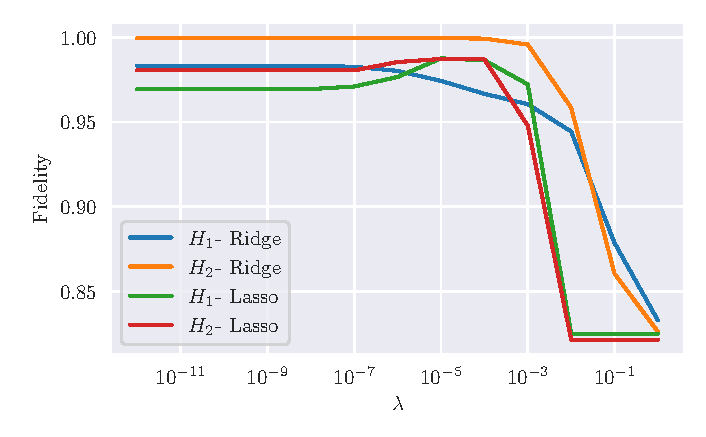
\includegraphics{figures/without_rz_ab_new.pdf}
        \caption{Fidelity as function of lambda for Ridge and Lasso regression using Hamiltonian $H_1$ and $H_2$. The number of imaginary time steps for the preparation were 10.}
        \label{fig:fidelity_vs_lmb}
    \end{center}
\end{figure}

\begin{figure}[h]
    \begin{center}
        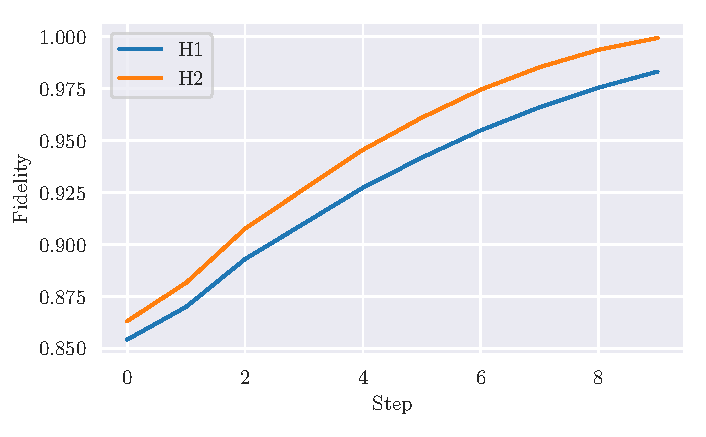
\includegraphics{figures/Fidelity_dynamic_lmb_without_rz_new.pdf}
        \caption{Fidelity as a function of imaginary time step using Ridge regression, varying the regularization parameter each step, choosing the parameter giving the numerical $\Dot{\omega}$ closest to the analytical $\Dot{\omega}$ without getting singular matrices.}
        \label{fig:fidelity_lambda_log_increament}
    \end{center}
\end{figure}

The Gibbs state results is summarized in \autoref{tab:fidelity_vs_ite}.

The final fidelity after 10 steps using a dynamical $\lambda$ resulted in fidelities of $0.98$ and $1.0$ using $H_1$ and $H_2$ respectively. 

\FloatBarrier
\subsection{Preparation of Gibbs states- Discussion}
Having a look at \autoref{fig:fidelity_vs_lmb} it shows that the highest fidelity between the analytical and approximated Gibbs state were received by $H_2$ using Ridge regression. For the $H_1$ Hamiltonian on the other hand, the highest fidelity were achieved by using Lasso regression for a small portion of $\lambda \in \log_{10}[-6,-3]$.

Since it seems that Ridge outperforms Lasso for small values of $\lambda$, Ridge where chosen as the regression method for the rest of the calculations. Another reason for choosing Ridge regression due to small values of $\lambda$ is that the smaller regularization, the closer the numerical $\Dot{\omega}$ will be to the $\Dot{\omega}$, as long as singular values are avoided. This is a different approach to how one normally would use Ridge regression in a supervised learning approach, where the regularisation value is used to prevent overfitting, while in this case, overfitting is desireable.

\autoref{fig:fidelity_lambda_log_increament} shows that having a dynamically changeable $\lambda$ during the evolution of Gibbs states provides approximated Gibbs states corresponding to fidelities close to $1$ for both $H_1$ and $H_2$. $H_1$ and $H_2$ resulted in fidelities of $0.98$ and $1.0$ respectively. The reason for $H_2$ being able to evolve into a more accurate Gibbs state is probably due to the four-qubit trial circuit being a better fit compared to the two-qubit trial circuit used in accordance to $H_1$. Fortunately due to the VarQBM being used for machine learning purposes the approximated Gibbs states do not require a $100\%$ match with the analytical states\cite{VQB:litteraturelist}, and will therefore work as noise in the dataset when the states are deviated by a small amount.

Using a set $\lambda$ seems to evolve the states approximately into the same Gibbs states as for the dynamically changeable $\lambda$, as long as $\lambda$ lays within a reasonable range. The dynamically changeable $\lambda$ will be used for further computations. The reason for this is that due to a dynamically changeable $\lambda$ finds the best regularisation each step, hence generalize easier to other systems.

\section{Generative Learning}
The VarQBM was used to generate probability distributions. The chosen learning parameters and final results will be revealed in this section.

\subsection{Parameter investigation}
Before the distributions were computed, some learning parameters had to be chosen. Firstly the learning rate were chosen. To get a reasonable estimate of the initial learning rate a method motivated by \cite{cyclical_lr} were used. The learning rate was increased exponentially after each epoch, resulting in an estimated learning rate of approximately $0.2$ for both Hamiltonians $H_1$ and $H_2$. The plot of the loss in addition to the increment learning rate can be seen in \ref{fig:lr_exp}.

\begin{figure}%
    \centering
    \hspace*{-0.1\textwidth}
    \subfloat[\centering]{{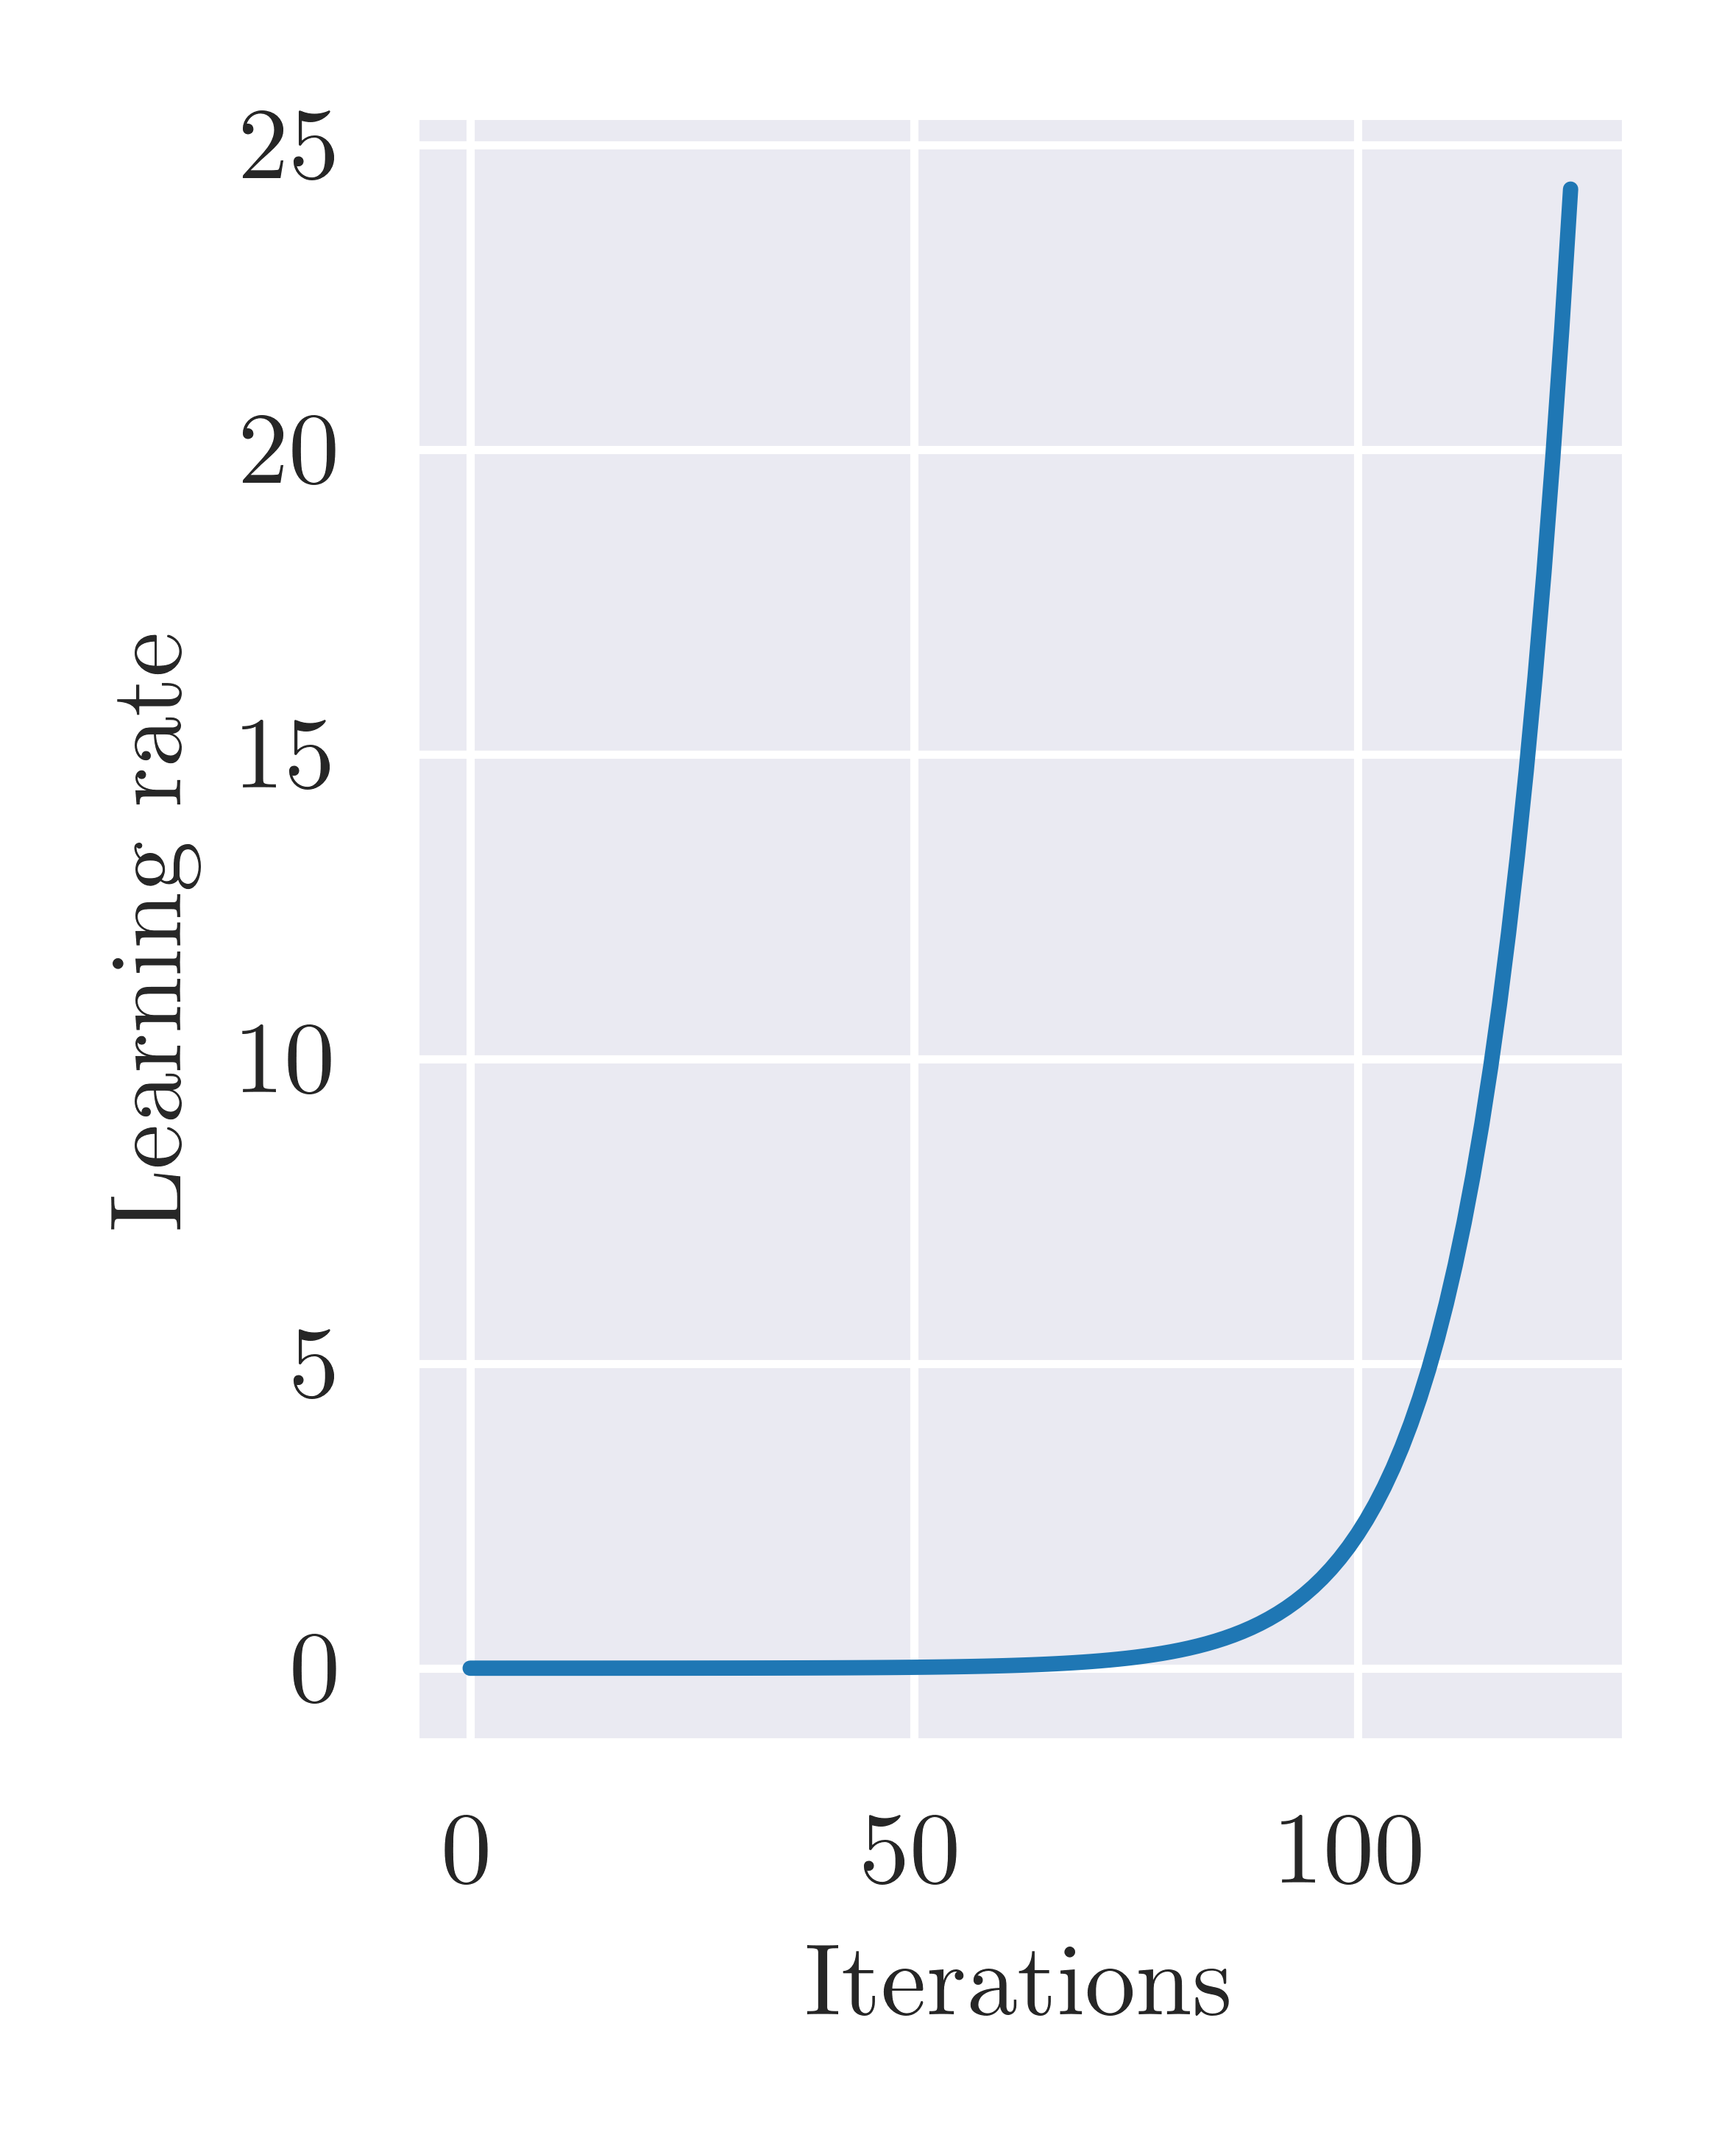
\includegraphics[width=0.6\textwidth]{figures/SGDitVSloss_hs.png} }}%
    %\qquad
    \subfloat[\centering]{{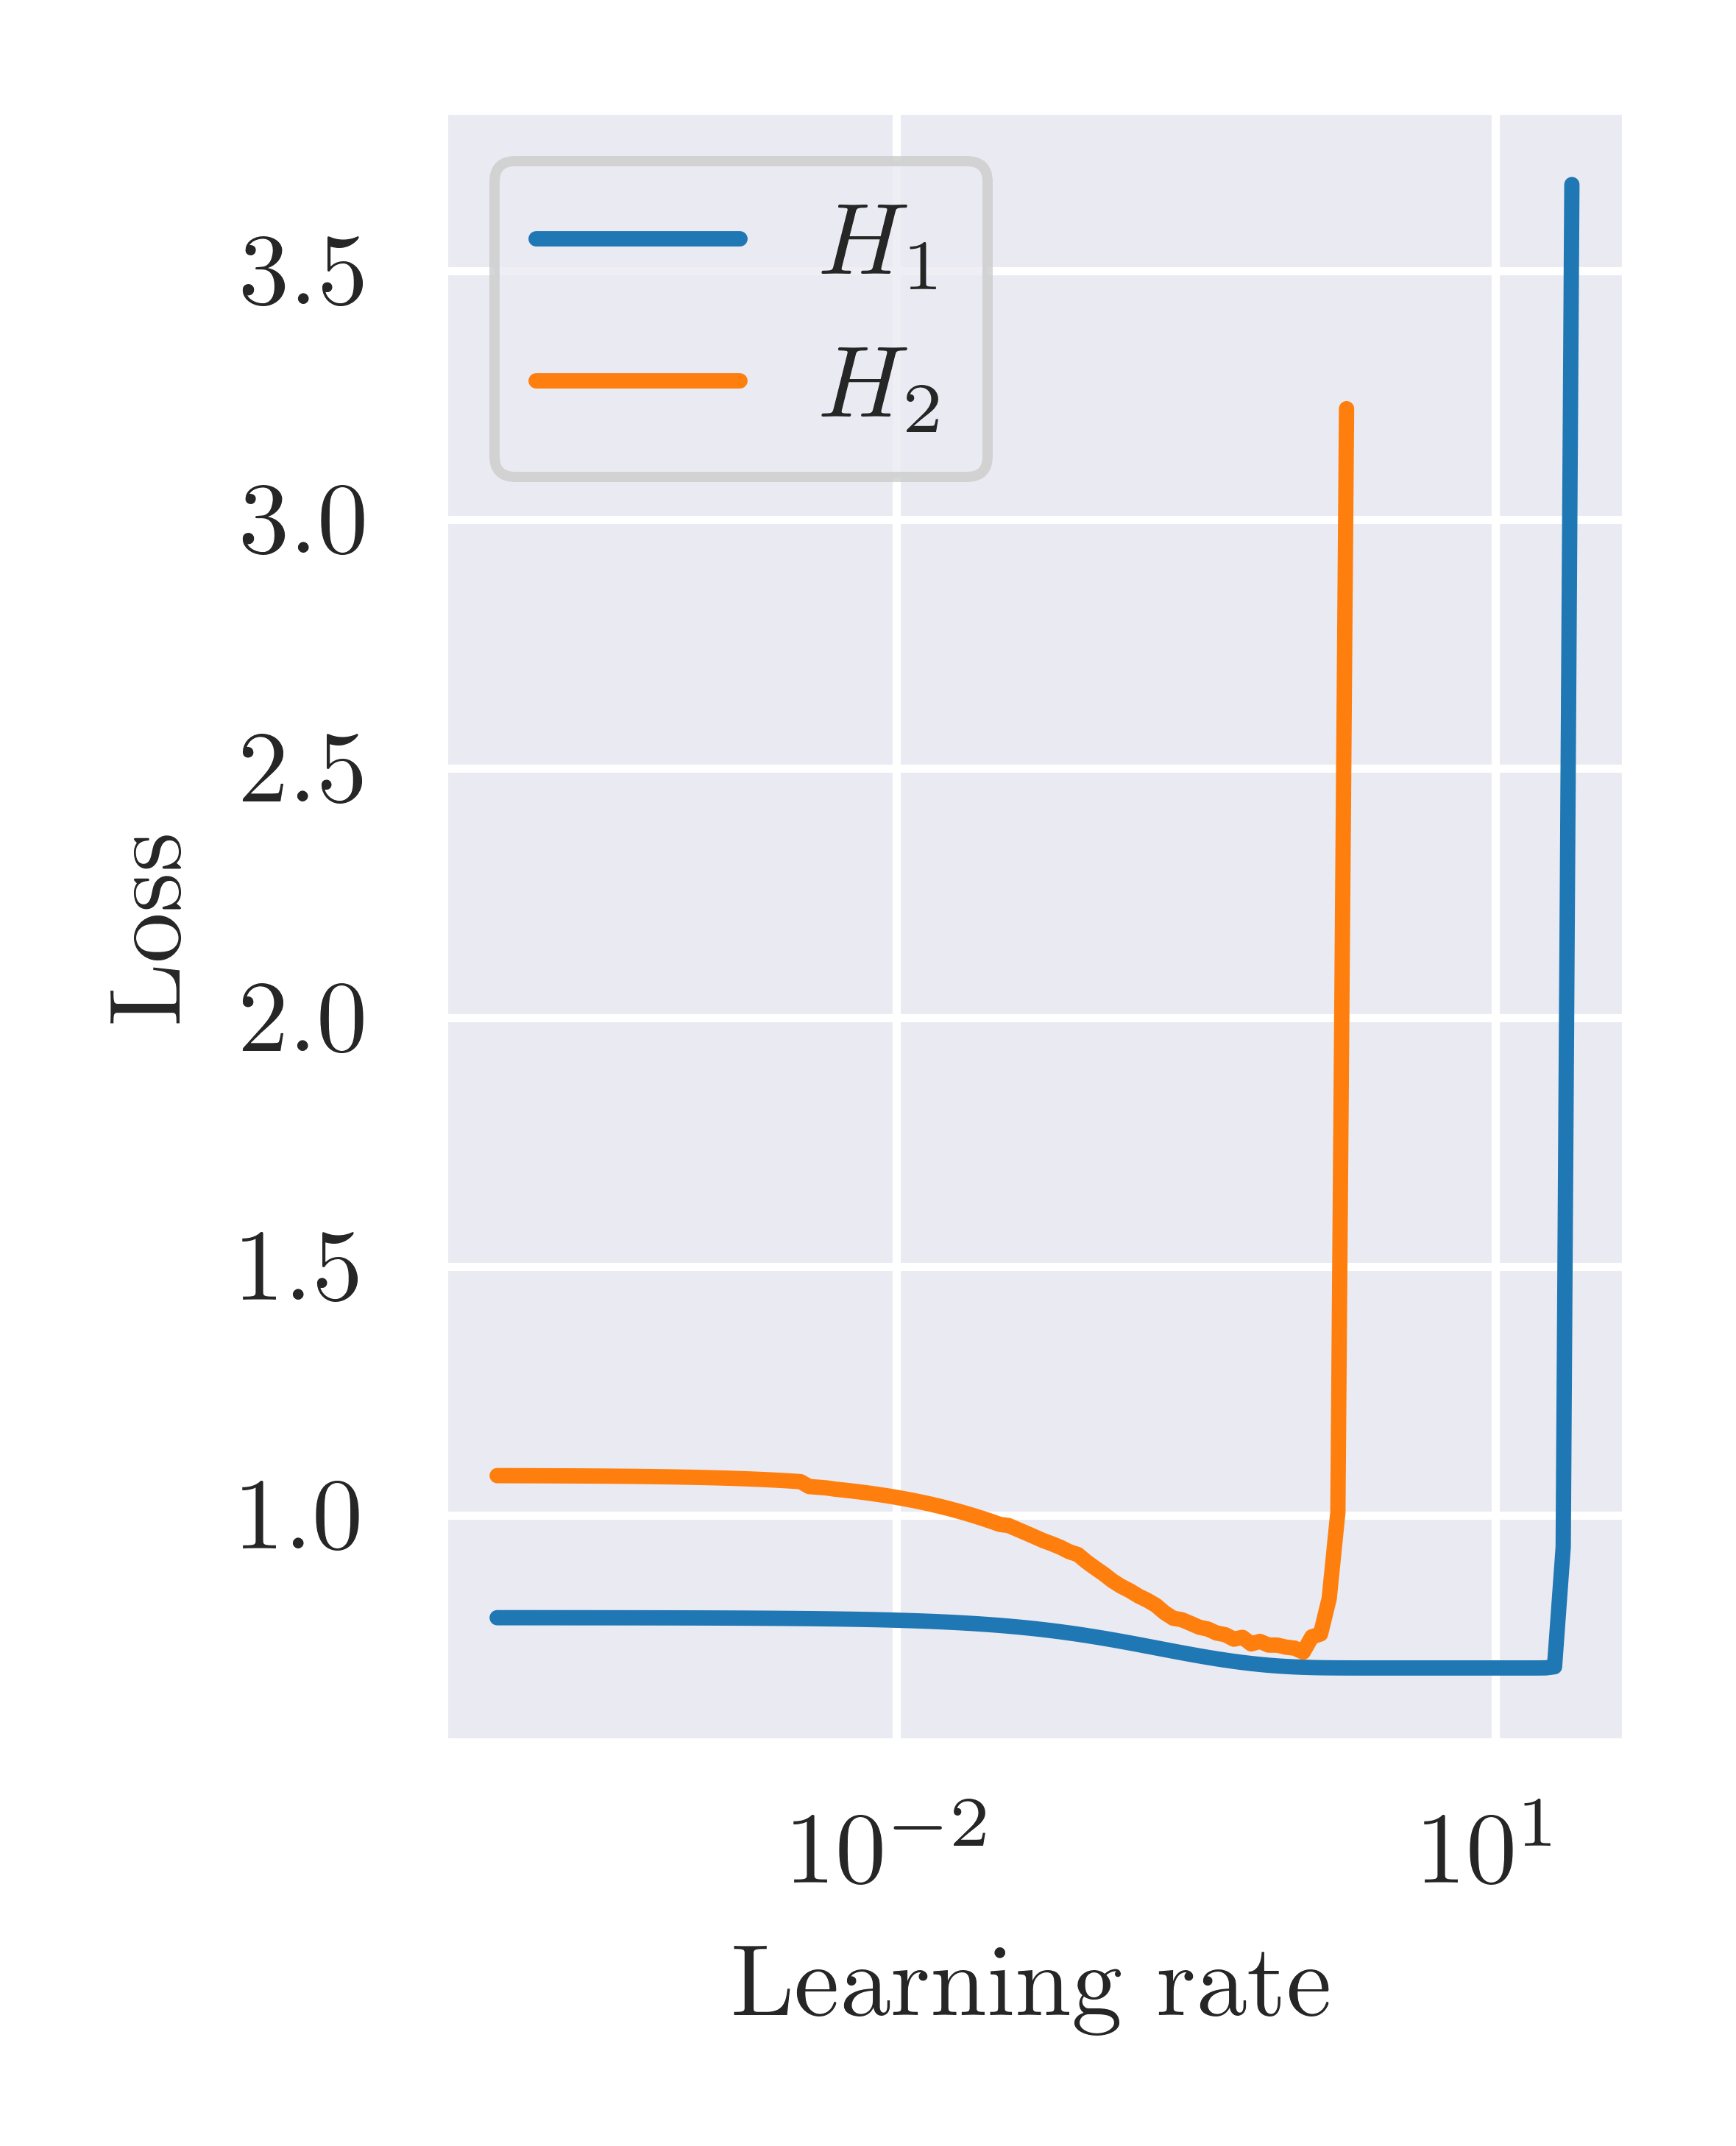
\includegraphics[width=0.6\textwidth]{figures/SGDlrVSloss_exp_SGDitVSloss_hs.png} }}%
    \caption{Learning rate investigation using SGD as the optimization technique. a) Increment of the learning rate as function of iterations applied to figure b). b) Loss as a function of increased learning rate}%
    \label{fig:lr_exp}%
\end{figure}

\autoref{fig:H1_loss_es} and \autoref{fig:loss_vs_it_vs_lr} shows how the learning rates and optimization technique applies to a $1$-qubit- and $2$-qubit Hamiltonian respectively.

\begin{figure}[h]
    \begin{center}
        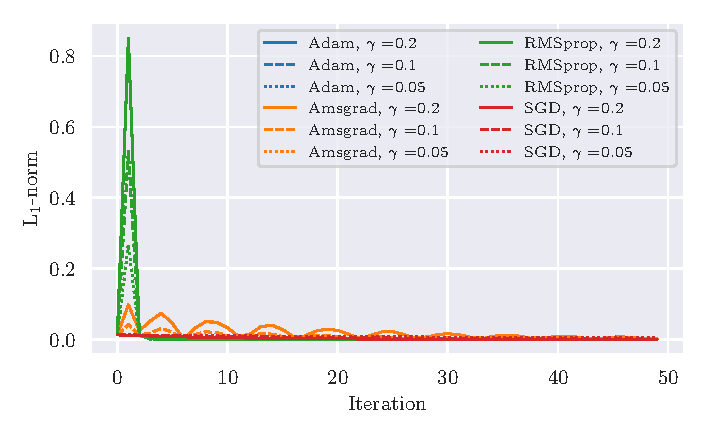
\includegraphics{figures/H1_ab_new_norm.pdf}
        \caption{Norm as function of iterations. Generating a probability distribution $[0.5, 0.5]$ using a 1-qubit Hamiltonian and a variety of optimization methods and learning rates. The norm is used instead of loss to perceive the trend easier. The norm is computed between the target distribution and the generated distribution. The ADAM optimizer overlaps with the AMSGrad optimizer.}
        \label{fig:H1_loss_es}
    \end{center}
\end{figure}

\todo[inline]{Plot again using a log scale}

\begin{figure}[h]
    \begin{center}
        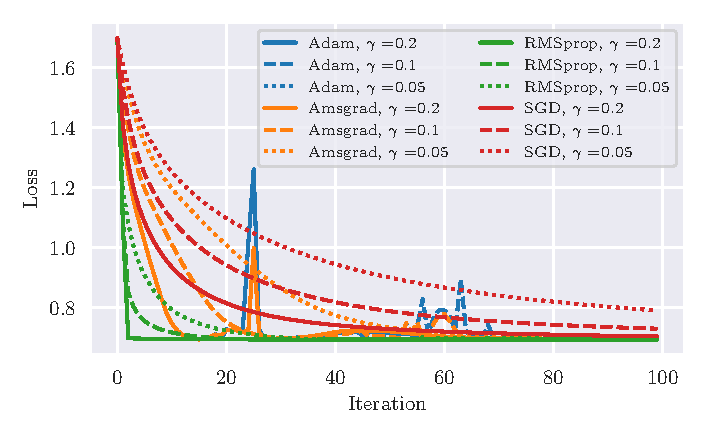
\includegraphics{figures/H2_ab_loss_linear.pdf}
        \caption{Loss as function of iterations. Recreating the Bell state using a 2-qubit Hamiltonian and a variety of optimization methods and learning rates.}
        \label{fig:loss_vs_it_vs_lr}
    \end{center}
\end{figure}

\todo[inline]{Plot again using a log scale}

\FloatBarrier
\subsubsection{Parameter investigation - Discussion}
\autoref{fig:lr_exp} argues that the optimal learning rate is 0.22, but this is taken as a roughly estimate, mainly due to the fact that the target distribution needless to say is constant during the whole training, in theory making the generated distribution a bit more identical to the target after each iteration, hence making it more difficult for the later iterations to have a large jump in decrement of loss before the learning rate gets to big. Even though this might even out due to the learning rate increasing and the gradient decreasing during training until the blowup of loss due to the enormous learning rate.

The estimation of the learning rate were taken into account and applied to different optimization techniques. \autoref{fig:H1_loss_es} and \autoref{fig:loss_vs_it_vs_lr} both argues that the optimal optimization method would be RMSProp due to the fastest converging towards a minimum. The learning rate on the other hand seem to be best being set to $0.2$ for the 2-qubit Hamiltonian, and quiet good for a 1-qubit Hamiltonian, but due to a large blowup at the start of the training of the 1-qubit Hamiltonian, a learning rate of $0.1$ where chosen.

The momentum parameter of the RMSProp optimization technique were investigated slightly showing that all momentum terms $m \in [0.6, 0.999]$ converged during training. The figure can be seen in \autoref{sec:third-app}. The momentum was set to $0.99$ for further computations. 

\FloatBarrier
\subsection{Generating probability distributions}

\begin{figure}[h]
    \begin{center}
        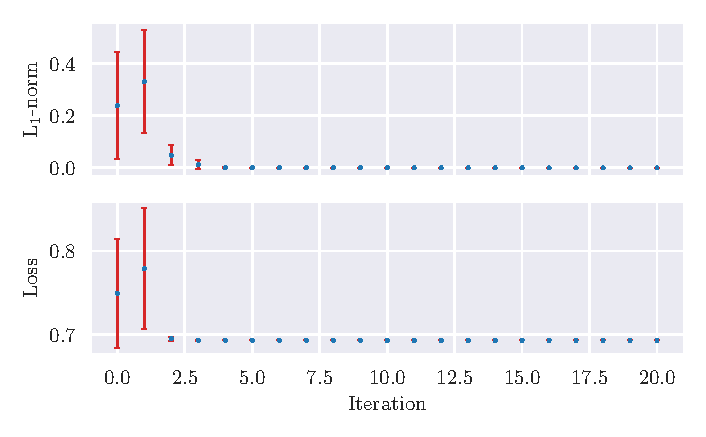
\includegraphics{figures/H1_ab_sub_10seeds.pdf}
        \caption{Generation of a probability distribution [0.5, 0.5] using a 1 qubit Hamiltonian. The quantum Boltzmann machine is fully visible. Loss and norm as a function og iteration steps. The plot represents the mean of 10 random seeds, and the bars represent the standard deviation.}
        \label{fig:nolabel}
    \end{center}
\end{figure}

\begin{figure}[h]
    \begin{center}
        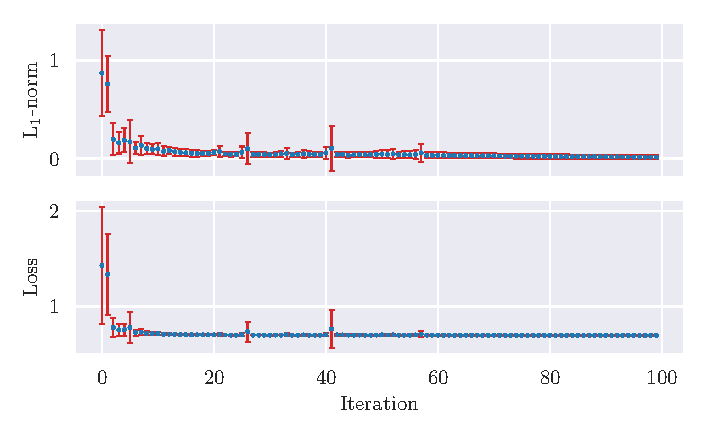
\includegraphics{figures/H2_ab_sub_10seeds.pdf}
        \caption{Too hard to see? Generation of a 2 qubit Hamiltonian. The quantum Boltzmann machine is fully visible. Loss and norm as a function of iteration steps. The plot represents the mean of 10 random seeds, and the bars represent the standard deviation.}
        \label{fig:nolabel}
    \end{center}
\end{figure}

\begin{figure}[h]
    \begin{center}
        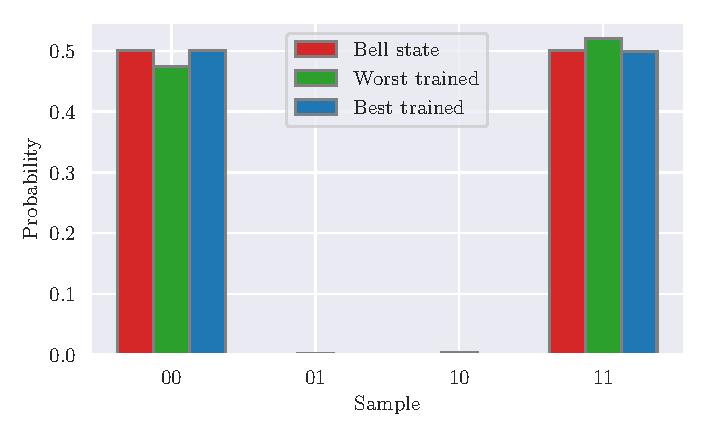
\includegraphics{figures/H2_abRMS_lr01m099bar_10seeds.pdf}
        \caption{Seems good}
        \label{fig:nolabel}
    \end{center}
\end{figure}

\FloatBarrier
\section{Discriminative Learning-Transaction dataset}
This section contains results regarding discriminative learning. Where The fraud dataset and 8x8 MNIST dataset were used.

\subsection{VarQBM: Input as bias}
In this section the input of the VarQBM were inserted according to \todo[inline]{Insert referal to the bias input section when the section is done}
\subsection{VarQBM: Neural Network feature engineering}
In this section the input of the VarQBM were inserted according to \todo[inline]{Insert referal to the neural network input section when the section is done}

Starts with initialization of weights in \autoref{fig:init_X_and_H}.

\begin{figure}%
    \centering
    \subfloat[\centering]{{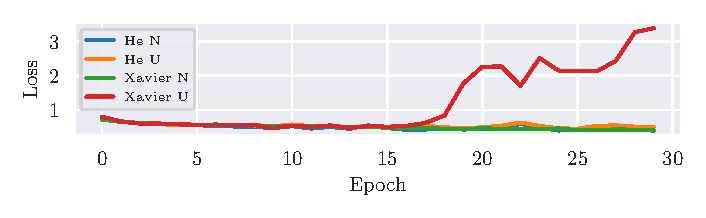
\includegraphics[width=\textwidth]{figures/loss_train12_2_sig_initialisationhhall.pdf} }}%
    \\
    \subfloat[\centering]{{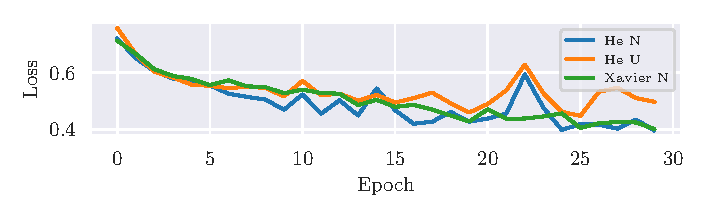
\includegraphics[width=\textwidth]{figures/loss_train12_2_sig_initialisationhh3.pdf} }}%
    \caption{Initialisation of weights. N is normal, U is uniform a) 4 different initialisations b) A better view of He normal, He uniform and Xavier normal}%
    \label{fig:init_X_and_He}%
\end{figure}

\begin{comment}
\begin{figure}
\centering
\begin{subfigure}[\centering]
   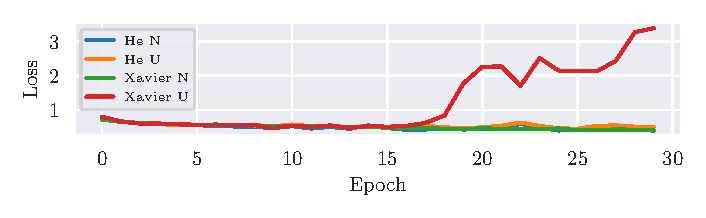
\includegraphics[width=1\textwidth]{figures/loss_train12_2_sig_initialisationhhall.pdf}
   \caption{}
  \end{subfigure}
\begin{subfigure}[\centering]
   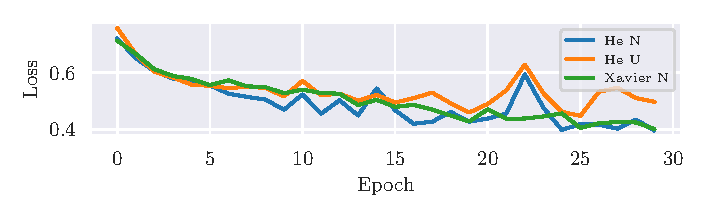
\includegraphics[width=1\textwidth]{figures/loss_train12_2_sig_initialisationhh3.pdf}
   \caption{}
\end{subfigure}
\caption{Le caption}
\end{figure}
\end{comment}

\begin{figure}%
    \centering
    \subfloat[\centering]{{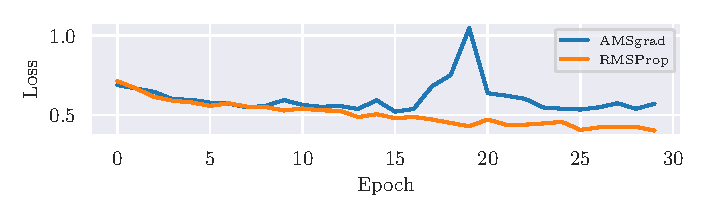
\includegraphics[width=\textwidth]{figures/loss_trainsig_12_2_lroptim_subH2.pdf} }}%
    \\
    \subfloat[\centering]{{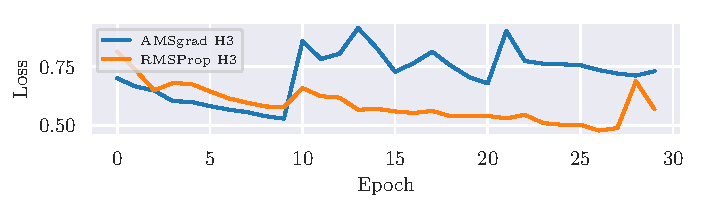
\includegraphics[width=\textwidth]{figures/loss_trainsig_12_2_lroptim_sub_H3.pdf} }}%
    \caption{Tested both H2 and H2.2 with AMSgrad and RMSProp, might remove this, cause it is not that relevant and but we'll what ends up in the thesis eventually.}%
    \label{fig:lr_exp}%
\end{figure}

\begin{figure}
    \begin{center}
        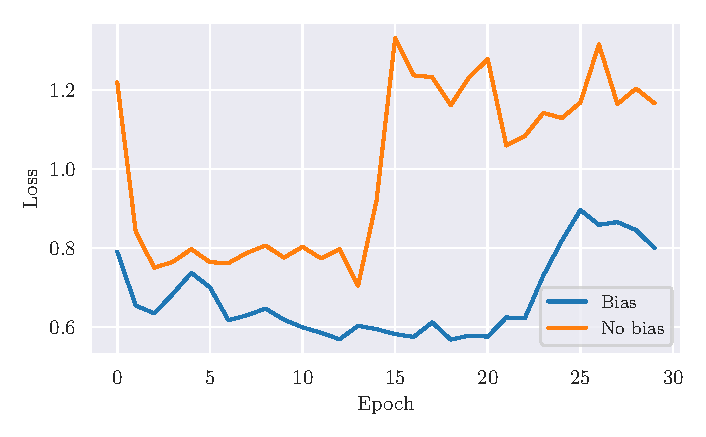
\includegraphics{figures/bias_12_2_50_samples.pdf}
        \caption{2 hidden layers with 12 hidden nodes each and sigmoid activation functions within the hidden layers, with and without bias initialized as 0.01 using 50 samples. The neural net is initialized using xavier normal initialisation.}
        \label{fig:4}
    \end{center}
\end{figure}

\begin{figure}
    \begin{center}
        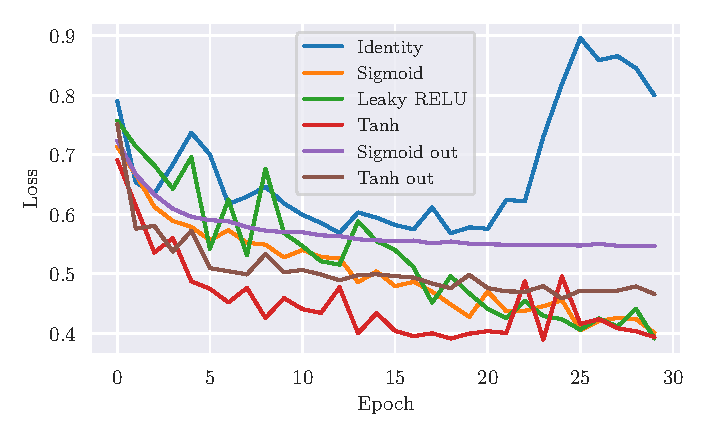
\includegraphics{figures/loss_activations_12_2_without_relu.pdf}
        \caption{2 qubit Hamiltonian with 1 hidden qubit, using a neural network of 2 hidden layers with 12 hidden nodes and bias, using 50 samples, computed using different activation functions.}
        \label{fig:3}
    \end{center}
\end{figure}


\begin{figure}
    \begin{center}
        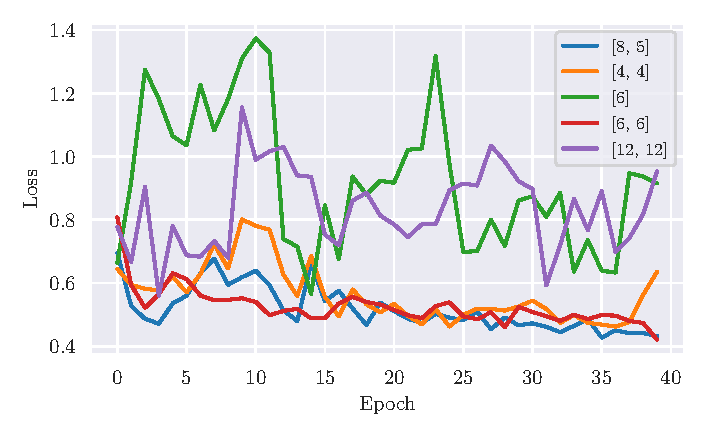
\includegraphics{figures/H2_NNsizes_tr_fraud.pdf}
        \caption{Layer sizes- Transaction dataset. 100 samples in all plots below}
        \label{fig:2}
    \end{center}
\end{figure}

\begin{figure}
    \begin{center}
        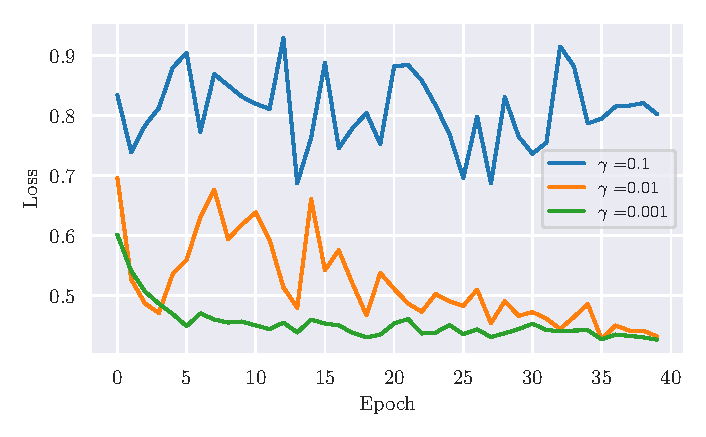
\includegraphics{figures/H2_lr_fraud_tr.pdf}
        \caption{Learning rate- Transaction dataset}
        \label{fig:1}
    \end{center}
\end{figure}

\subsection{Restricted Boltzmann machine}
Solving the transaction data using a restricted Boltzmann machine with logistic regression layer on top.

First set the amount of hidden nodes. The accuracy were plotted as a function of hidden nodes using default values of scikit-learn. Here all samples were labeled as non fraud, so 30 hidden nodes were chosen.

Then an exhaustive search over specified parameter values were done searching across the following values:

\begin{center}
\begin{tabular}{l l}
 Learning rate: & 0.001, 0.005, 0.01, 0.05, 0.1, 0.5 \\ 
 Batch size & 1, 2, 5, 10  \\  
 Logistic hyperparameter C & 0.5, 1, 5, 10, 50, 100, 500    
\end{tabular}
\end{center}

Best parameters found from grid search performed was learning rate of 0.001, batch size of 1 and hyperparameter C 0.5.

The cofusion matrix can be seen in \autoref{fig:transaction_cm}. Easy to see that the RBM still labels all samples as fraud.
\begin{figure}
    \begin{center}
        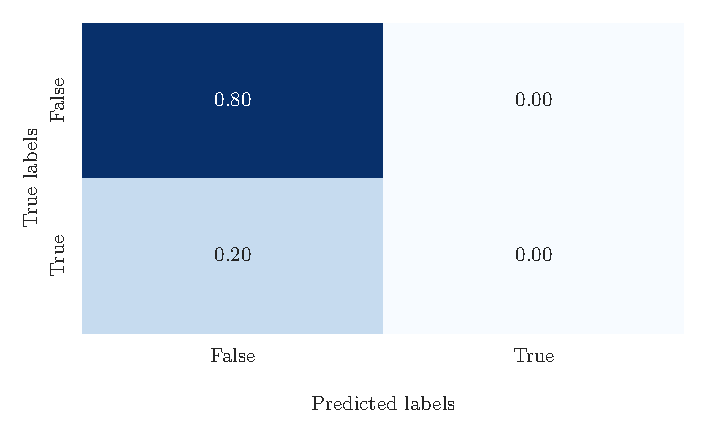
\includegraphics{figures/CMfraud.pdf}
        \caption{RBM- confusion matrix- Transactions. All samples are classified as fraud}
        \label{fig:transaction_cm}
    \end{center}
\end{figure}

\subsection{Transaction data scores}
The final runs achieved using the classical RBM and the VarQBM with and without neural network feature engineering can be seen in \autoref{tab:final_results_table_transaction}

\begin{table}[H]
\centerline{
\begin{tabular}{ ccccc } 
\toprule
 Model & Accuracy & Precision & Recall & $F_1$ score\\ 
\midrule
 VarQBM bias encoding & 0.69 & 0.76 & 0.69 & 0.71 \\
 \textbf{VarQBM NN encoding} &  \textbf{0.82} & \textbf{0.81} & \textbf{0.82} & \textbf{0.78} \\
 RBM &  0.80 & 0.64 & 0.80 & 0.71\\ 
\bottomrule
\end{tabular}}
\caption{Final results, 400 samples, 50 epochs, 0.01}
\label{tab:final_results_table_transaction}
\end{table}

\section{Discriminative Learning-Handwritten image recognition}

Choosing to continue with some of the found parameters from the transaction investigation. Including a bias, if it is better without a bias in the network, it will reduce to 0 during training. In addition the Xavier N initialisation and tanh as activation function within the network are used.

\subsection{VarQBM: Input as bias}
\todo[inline]{Run computations when input is inserted the normal way}
\subsection{VarQBM: Neural Network feature engineering}

\begin{figure}
    \begin{center}
        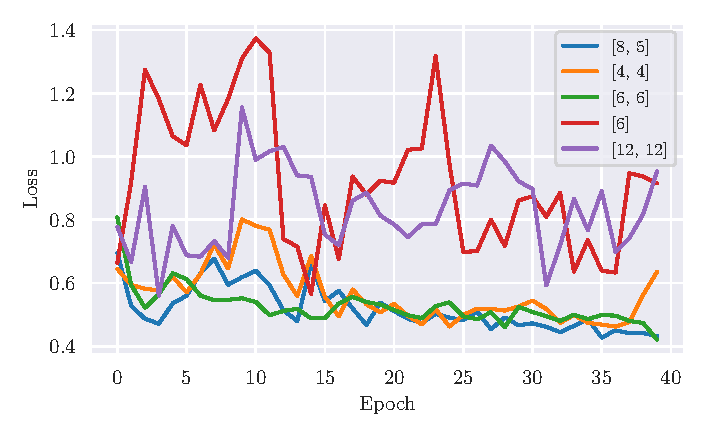
\includegraphics{figures/H2_NNsizes_tr.pdf}
        \caption{Layer sizes- Digit dataset}
        \label{fig:loss_epoch_layers}
    \end{center}
\end{figure}

\begin{figure}
    \begin{center}
        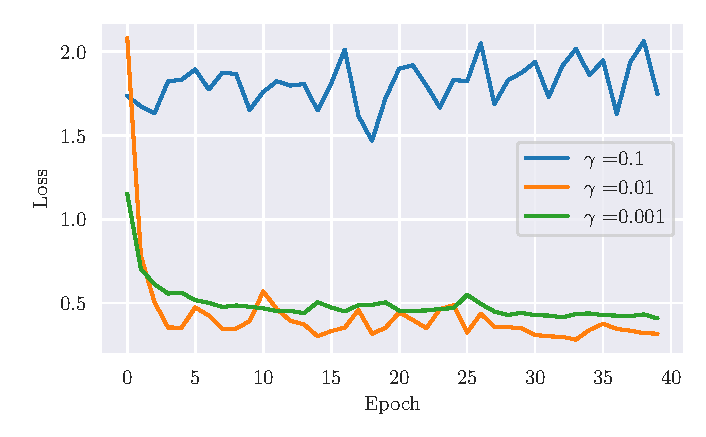
\includegraphics{figures/H2_lr_mnist_tr.pdf}
        \caption{Learning rate- Digit dataset}
        \label{fig:loss_ep_gamma}
    \end{center}
\end{figure}

\subsection{Restricted Boltzmann machine}
Solving the digit dataset using a restricted Boltzmann machine with logistic regression layer on top.

First set the amount of hidden nodes. The accuracy were plotted as a function of hidden nodes using default values of scikit-learn. The results cn be seen in figure \autoref{fig:hn_vs_acc}. The choosen amount of hidden nodes was 30.

\begin{figure}
    \begin{center}
        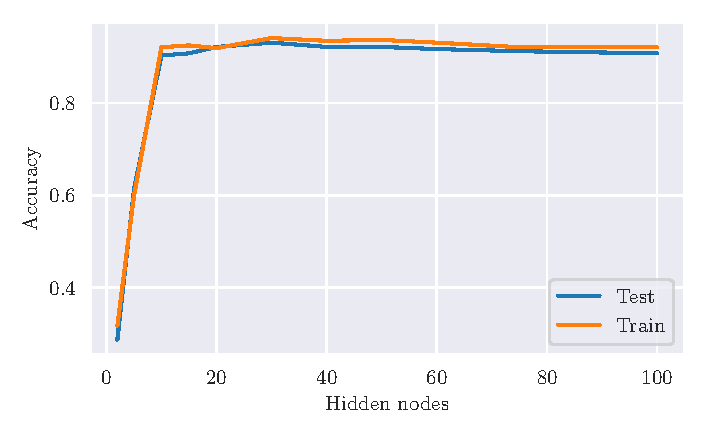
\includegraphics{figures/rbm_h_vs_acc_digit2.pdf}
        \caption{RBM - Accuracy as a function of the number of hidden nodes- Transactions}
        \label{fig:hn_vs_acc}
    \end{center}
\end{figure}

Then an exhaustive search over specified parameter values were done searching across the same values as for the transaction dataset in \todo[inline]{Add referral to the table of gridsearch parameters}

Best parameters found from grid search performed was learning rate of 0.05, batch size of 2 and hyperparameter C of 100.

The cofusion matrix can be seen in \autoref{fig:digit_cm}.
\begin{figure}
    \begin{center}
        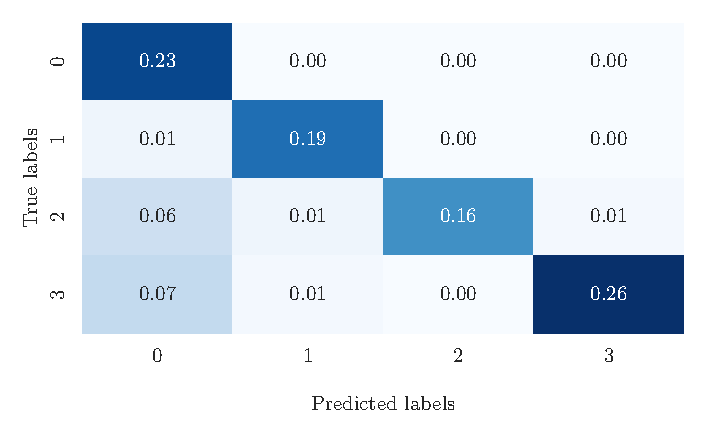
\includegraphics{figures/CMmnist.pdf}
        \caption{RBM- confusion matrix- Digit dataset. }
        \label{fig:digit_cm}
    \end{center}
\end{figure}

RBM with $0.99$ accuracy on digit dataset(Only four classes.

\subsection{Handwritten image recognition scores}
The final runs achieved using the classical RBM and the VarQBM with and without neural network feature engineering can be seen in \autoref{tab:final_results_table_digits}

\begin{table}[H]
\caption{Final results, 400 samples, 50 epochs, 0.1lr. weighted precision, recall and F1 score, NN layer: [8,5]}
\centerline{
\begin{tabular}{ ccccc } 
\toprule
 Model & Accuracy & Precision & Recall & $F_1$ score\\ 
\midrule
 VarQBM bias encoding & 0.56 & 0.54 & 0.56 & 0.53 \\
 VarQBM NN encoding &  0.73 & 0.85 & 0.73 & 0.65 \\
 \textbf{RBM} &  \textbf{0.98} & \textbf{0.98} & \textbf{0.98} & \textbf{0.98} \\
\bottomrule
\end{tabular}}
\label{tab:final_results_table_digits}
\end{table}

\section{MNIST scores}
The final runs achieved using the classical RBM and the VarQBM with neural network feature engineering can be seen in \autoref{tab:final_results_table_mnist}
\begin{table}[H]
\caption{28x28 pixels, 4 classes. Final results, 400 samples, 50 epochs, 0.01lr. weighted precision, recall and F1 score}
\centerline{
\begin{tabular}{ cccccc } 
\toprule
 Model & NN encoding &Accuracy & Precision & Recall & $F_1$ score\\ 
\midrule
 VarQBM & [32,32]& 0.83 & 0.86 & 0.83& 0.84 \\
 VarQBM & [123,19] & 0.33 & 0.11 & 0.33 & 0.16 \\
 \textbf{RBM} & & \textbf{0.91} & \textbf{0.91} & \textbf{0.91} & \textbf{0.91} \\
\bottomrule
\end{tabular}}
\label{tab:final_results_table_mnist}
\end{table}



\end{document}